%\chapter{Image Style Transfer}\chlbl{image_style_transfer}
%In the field of image style transfer\sidecite{Gatys_Ecker_Bethge_2015}, such correlations are used to generate images.
%An image is created based on two images, one image providing the content (i.e. the ``content-image'') and the other image providing the style (i.e. the ``style-image'').
%To generate the content of the image, a random image can be fed into the model and a simple distance-based loss function such as the Euclidean norm can be used to calculate the difference between the model output and the content-image.
%Over time, the model would learn to output the content-image.
%However, only the content from the content-image and not its style is needed.
%A solution to this problem is using Convolutional feature maps\sidenote{a convolutional layer can have multiple filters (i.e. channels), each filter produces a convolutional feature map} as they capture spatial information of an image well, while containing only little style information.
%Therefore, the distance loss is not calculated between the content-image and the model output but between the feature maps of the content-image and the output image.

%The second task is to transfer the style from the style-image to the model output.
%The style of an image can be described by correlations across the different feature maps.
%This information about the image style can be calculated with a Gram matrix.
%A Gram matrix is the dot product\sidenote{the dot product between two vectors can be seen as similarity metric; it gets bigger if two vectors are more similar} of the flattened feature vectors from a convolutional feature map (i.e. the dot product between all channels of a convolutional layer's output).
%For example, a convolutional layer could have multiple channels. The first channel could have a high activation for black and white stripes in horizontal direction while the second channel could have a high activation for black and white stripes in vertical direction. If both channels activate together for the same input and thus have a high correlation, there is a high possibility that the image might contain the style of a chessboard (i.e. black and white checkered). A third channel, for example, could have a high activation for eyes. If this channel has a low correlation with the first channel but a high correlation with the second channel (i.e. black and white stripes in vertical direction), the input image might contain the face of a zebra and thus capture a ``zebra-style''.
%Similar to the content-transfer, a distance loss such as the Euclidean distance can be used to compare the Gram matrices of the style-image and the output-image.
%Thus, it is compared if the output-image has the same style as the style-image.

%In summary, the content is transferred by comparing entire convolutional layer output and the style by comparing the correlations between the feature maps of a convolutional layer output (i.e. by comparing gram matrices).

%\pagebreak
%\chapter{Design Decisions}\chlbl{design_decisions}
%There exists a variety of possibilities how self-organization of the network architecture can be implemented.
%However, this thesis is of course limited in time and resources an thus not all of them can be investigated.
%Therefore, a promising direction of research had to be defined at the beginning and followed afterwards.

%As a constraint it was defined that (i) a network without dynamics is developed and (ii) self-organization takes place across multiple layers.
%A network without dynamics is used because Deep Learning works very well for pattern recognition and the data analyzed by the computer is mostly static.
%Dynamic networks usually have poorer performance and use special algorithms to convert static data such as images into dynamic time-related signals (c.f. Section \secref{self_org_spiking}).
%Applying self-organization across multiple layers rather than just adding lateral connections in one layer is preferred as this allows the network to form more complex structures and thus to use the whole potential of self-organisation.

%This thesis is strongly inspired by the paper ``Natural Intelligence'' \sidecite{von_der_Malsburg_Stadelmann_Grewe_2022} (c.f. Section \secref{natural_intelligence}).
%The most relevant findings in this work are:

%\begin{itemize}
%  \item The brain is highly structured
%  \item Self-organization is the most promising approach to achieve natural intelligence. It loops between activity and connectivity
%  \item Self-organization forms net fragments, one neuron can be part of multiple fragments
%  \begin{itemize}
%    \item An object can be represented by multiple net fragments
%    \item A hierarchy of features can be represented by nested net fragments
%  \end{itemize}
%  \item The self-organizing process has to start from an already established coarse structure
%  \item There exists many alternative pathways in the network
%\end{itemize}

%However, it is unclear how these findings and hypotheses from the field of neuroscience can be implemented in an algorithm.
%To create a self-organizing neural network, the following mechanisms are particularly relevant: The design of the initial architecture, the allowed architecture modifications (removing and adding neurons and/or connections), the type of neurons, and the definition of the learning algorithm.
%These aspects are discussed hereafter.

%\begin{description}
%   \item[Design of initial architecture] The initial architecture should exhibit a good inductive bias from the start so that the network can learn (something meaningful). Current approaches also start from much bigger architectures and reduce their size by up to a thirty-fold \sidecite{Pedersen_Risi_2021} (c.f. Section \secref{self_org_related}) or grow the architecture from a single neuron \sidecite{Raghavan2019NeuralNG} (c.f. Section \secref{self_org_spiking}) by using self-organisation.
%   \item[Architecture modifications] The architecture can be modified in several ways. For example, from a more global perspective, the network can grow, shrink, split into sub-networks\sidenote{this is related to ensemble approaches TODO: add source}, or multiple sub-networks can re-organize into one network. From a local perspective, connections can be created or removed within the same layer (lateral connections) or between subsequent layer. Moreover, connections can be used to skip on or several layers (residual connections), or connections can be recurrent to a previous layer. Furthermore, besides modifying single connections and neurons, complete blocks of neurons can be added or removed. This includes for example layers, mathematical functions like pooling operations, or pre-defined modules consisting of several layers.
%   \item[Type of neurons] As described above, no dynamic (i.e. spiking) neurons are employed. The classical neurons multiply the input \(\boldsymbol{x}\) by a weight vector \(\boldsymbol{w}\), add a bias \(\boldsymbol{b}\) and calculate the output with a non-linear activation of this sum (c.f. Section \secref{ann}). However, recent architectures replace such classical neurons with more complex units. For example, Kirsch and Schmidhuber \sidecite{kirsch2021meta} (c.f. Section \secref{self_org_related}) use tiny RNNs with shared parameters as neurons. Such neurons are able to learn learning algorithms which are equivalent to back-propagation.
%   \item[Learning algorithm] ... (see learning to learn or Hebbian based on input covarinace or learning based on target label (e.g. enforce some distinction in neurons covariance matrix depending on label))
%\end{description}


\pagebreak
\chapter{Experiments Hebbian Learning}\chlbl{exp_hebb_learning}
Hebbian learning is the most plausible learning algorithm from a biological point of view (c.f. \secref{hebbian}).
Because of the high plausibility and the self-organising property, the effectiveness of Hebbian learning for extracting image representations was investigated in multiple preliminary experiments.
In this thesis, it was observed that Hebbian learning works well for tiny networks but does not scale to larger networks or more complex datasets.
Of course, it cannot be concluded from these preliminary experiments that Hebbian learning cannot be used to train networks for extracting image representations on a larger scale.
However, it was found that it is not trivial and that applying the Hebbian learning rule on modern architectures is not sufficient to obtain good feature extractors.

When the classical Hebbian learning rule as described in \eqref{hebb_1} is used, the weights in the network become symmetric.
As a result, the model does not learn different features, and the image representations are very poor.
This symmetry can be broken using the ABCD-Hebbian learning rule \sidecite{Niv_Joel_Meilijson_Ruppin_2001}.
The ABCD learning rule calculates the weight update \(\Delta w_{ij}\) from neuron \(i\) to neuron \(j\) based on the pre-synaptic activity \(a_i\) of neuron \(i\) and post-synaptic activity \(a_j\) of neuron \(j\) as follows:

\begin{align}\eqlbl{hebb_abcd}
	\Delta w_{ij} = \eta_{w_{ij}} \cdot (A_{w_{ij}} a_ia_j + B_{w_{ij}} a_i + C_{w_{ij}} a_j + D_{w_{ij}})
\end{align}

where \(\eta_{w_{ij}}\) is a weight-specific learning rate, \(A_{w_{ij}}\) is a correlation coefficient, \(B_{w_{ij}}\) is a presynaptic coefficient, \(C_{w_{ij}}\) is a postsynaptic coefficient, and \(D_{w_{ij}}\) is a bias coefficient.
The bias coefficient \(D_{w_{ij}}\) can be interpreted as an individual inhibitory or excitatory bias of each connection in the network.
As proposed by Najarro and Risi \sidecite{NEURIPS2020_ee23e7ad}, the coefficients are learnt through an evolution strategy \sidecite{Salimans_Ho_Chen_Sidor_Sutskever_2017}.
The symmetry is broken by applying the ABCD learning rule, and the image representations improve.
However, image processing networks usually consist of many parameters and using an evolutionary strategy to find them does not scale well.
Thus, the author's impression is that current Hebbian learning rules are only of limited use for learning deep learning-based image extraction networks.


\subsection{Hebbian Pruning}
Hebbian learning has not led to good image representations.
However, it was found that Hebbian learning might be promising to prune models trained with end-to-end backpropagation of error:
In the following, Hebbian learning is used to push weights between neurons towards zero or to set them exactly to zero.

Therefore, a neural network consisting of two convolutional layers, followed by a max-pooling layer, and three linear layers is used.
The convolutional layers have a kernel size of $3\times3$ and a stride of $1$. The first convolutional layer has $32$ channels, and the second has $64$ channels.
The max-pooling layer has a kernel size of $2\times2$ and thus halves the size of the feature map. 
The activation map is then flattened and fed into $3$ fully connected layers with an output size of \(1024\), \(128\), and \(10\), respectively.
Between each layer, ReLU activations are employed.
The network is visualized in \figref{hebb_pruning}.

\begin{figure}[h]
    \centering
    \resizebox{0.99\textwidth}{!}
{
	\begin{tikzpicture}
		\tikzstyle{connection}=[ultra thick,every node/.style={sloped,allow upside down},draw=\edgecolor,opacity=0.7]
\tikzstyle{copyconnection}=[ultra thick,every node/.style={sloped,allow upside down},draw={rgb:blue,4;red,1;green,1;black,3},opacity=0.7]


\pic[shift={(0,0,0)}] at (0,0,0) 
    {Box={
        name=conv1,
        caption=Conv + ReLU,
        xlabel={{1, }},
        zlabel=32,
        fill=\ConvColor,
        height=16,
        width=4,
        depth=16
        }
    };


\pic[shift={(3,0,0)}] at (0,0,0) 
    {Box={
        name=conv2,
        caption=Conv + ReLU,
        xlabel={{32, }},
        zlabel=64,
        fill=\ConvColor,
        height=16,
        width=8,
        depth=16
        }
    };


\draw [connection]  (conv1-east)    -- node {\midarrow} (conv2-west);


\pic[shift={ (0,0,0) }] at (conv2-east) 
    {Box={
        name=pool1,
        caption= ,
        fill=\PoolColor,
        opacity=0.5,
        height=8,
        width=1,
        depth=8
        }
    };


\pic[shift={(4,0,0)}] at (pool1-east) 
    {Box={
        name=fcn1,
        caption=Hebb. Pruning + ReLU,
        xlabel={{" ","dummy"}},
        zlabel=1024,
        fill=\SoftmaxColor,
        opacity=0.8,
        height=3,
        width=3,
        depth=100
        }
    };


\draw [connection]  (pool1-east)    -- node {\midarrow} (fcn1-west);


\pic[shift={(2,0,0)}] at (fcn1-east) 
    {Box={
        name=fcn2,
        caption=Hebb. Pruning + ReLU,
        xlabel={{" ","dummy"}},
        zlabel=128,
        fill=\SoftmaxColor,
        opacity=0.8,
        height=3,
        width=3,
        depth=50
        }
    };


\draw [connection]  (fcn1-east)    -- node {\midarrow} (fcn2-west);


\pic[shift={(2,0,0)}] at (fcn2-east) 
    {Box={
        name=fcn3,
        caption=FCN + Softmax,
        xlabel={{" ","dummy"}},
        zlabel=10,
        fill=\SoftmaxColor,
        opacity=0.8,
        height=3,
        width=3,
        depth=25
        }
    };


\draw [connection]  (fcn2-east)    -- node {\midarrow} (fcn3-west);

\end{tikzpicture}
}
    \caption[Hebbian pruning network]{The network architecture used to perform Hebbian-based weight pruning.}
    \figlbl{hebb_pruning}
\end{figure}

The model is trained to classify digits with backpropagation of error on the MNIST dataset \cite{Lecun_Bottou_Bengio_Haffner_1998}.
Adam \sidecite{Kingma2015AdamAM} is used as optimisation algorithm to minimise the negative log-likelihood (NLL) loss.
The mini-batch size is \(32\) and the learning rate is \(5\cdot 10^{-4}\).
When the loss reaches a plateau, the learning rate is reduced to \(1\cdot 10^{-4}\).

After the model is trained, the first two fully connected layers within the network are pruned with Hebbian learning:
The \emph{first} Hebbian-based method proposed pushes the weights between neuron \(i\) and neuron \(j\) towards \(0\) if \(i\) and \(j\) have a low correlation within a mini-batch.
Therefore, a mini-batch is sampled, and the correlation between all neurons is calculated for each sample.
if the correlation is below \(0.02\) for at least \(20\%\) of the samples (i.e. \(7\) samples or more for a mini-batch size of \(32\)), the weight is reduced:
\begin{align}\eqlbl{hebb_towards_0}
	\Delta w_{ij} = - \eta_H \cdot w_{ij}
\end{align}
\begin{align}\eqlbl{hebb_towards_00}
	w_{ij} := w_{ij} + \Delta w_{ij}
\end{align}
%
where \(\eta_H\) is the Hebbian learning rate set to \(1\cdot 10^{-5}\).

The \emph{second} Hebbian-based method proposed pushes some weights exactly to \(0\) while all other weights remain the same.
During an epoch, the correlation between neurons \(i\) and \(j\) is measured for each weight \(w_{ij}\).
Afterwards, the weights with the lowest correlations are set to \(0\).
How many weights are set to \(0\) is a hyper-parameter that has to be specified in advance.


\subsection{Results}
For both methods, the model is trained on the MNIST training dataset \cite{MNIST}, and the weights are frozen.
Afterwards, the weights are pruned based on the MNIST training dataset and evaluated on the MNIST and MNIST-C\sidenote{MNIST-C is a corrupted version of MNIST and well suited to measure model robustness} \cite{Mu_Gilmer_2019} test dataset.
The \emph{first} Hebbian-based method can further improve the results even after the training has converged, as shown in \tabref{nll_hebb_pruning}.


\begin{table}[h] 
    \centering
	 \begin{tabular}{l c c} 
    	%\hline
    	 & \textbf{NLL-Loss} & \textbf{NLL-Loss} \\
        \textbf{Dataset} & \textbf{without Hebbian Updates} & \textbf{with Hebbian Updates}\\
        \hline
        MNIST & \(0.05314\) & \(0.03386\) \\
        MNIST-C & \(0.6013\) & \(0.4766\) \\
         & & \\
        %\hline
    	 &\textbf{Accuracy} & \textbf{Accuracy} \\
        \textbf{Dataset} & \textbf{without Hebbian Updates }& \textbf{with Hebbian Updates}\\
        \hline
        MNIST & \(98.94\%\) & \(99.31\%\) \\
        MNIST-C & \(88.74\%\) & \(89.94\%\) \\
        %\hline
    \end{tabular}
    \caption[NLL loss of the Hebbian pruning network]{NLL loss of the model before and after the \emph{first} Hebbian-based pruning method.}
    \tablbl{nll_hebb_pruning}
\end{table}

The NLL loss on the MNIST test dataset decreases from \(0.05314\) to \(0.03386\), while the loss on the MNIST-C test dataset decreases from \(0.6013\) to \(0.4766\).
Furthermore, the accuracy increases roughly by $1.2\%$ on MNIST-C, which is remarkable, considering that the model has been trained with gradient descent until convergence and only the weights are reduced after training (without further parameter updates).
It also has to be considered that this is only a preliminary experiment, and this method most likely can be further improved.
Thus, this experiment indicates that Hebbian could be used as a post-training step to improve robustness by reducing the model's weights.

\begin{figure}[h]
    \centering
    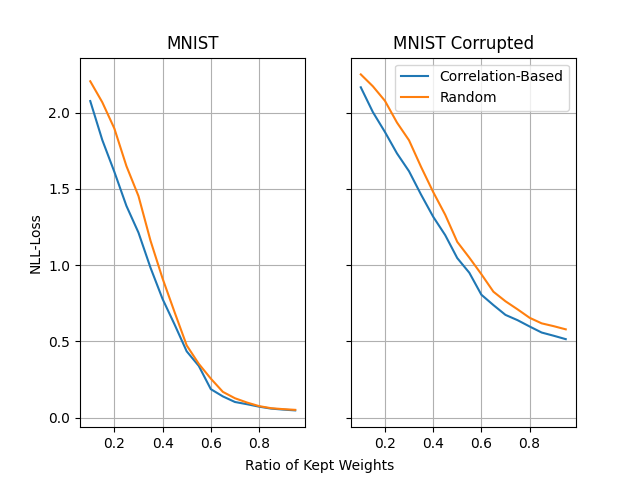
\includegraphics[width=0.79\textwidth]{loss_hebb_pruning}
    \caption[NLL loss of the Hebbian pruning network]{The NLL loss of the \emph{second} Hebbian-based pruning method compared to removing random weights. The y-axis shows the loss, while the x-axis shows the ratio of weights kept. }
    \figlbl{hebb_prune}
\end{figure}

The \emph{second} Hebbian-based method sets weights between neurons with a low correlation to \(0\).
The network trained with back-propagation has an accuracy of \(98.94\%\) on MNIST.
By setting up to \(40\%\) of the weights to \(0\), the accuracy remains above \(>98\%\).
Setting weights to \(0\) can make the network smaller and more efficient \sidecite{Liang_Glossner_Wang_Shi_Zhang_2021}.
Furthermore, it leads to sparse representations that can improve robustness.
\figref{hebb_prune} visualizes the loss of the \emph{second} Hebbian-based method for different ratios of kept weights.
Furthermore, the correlation-based method is compared to randomly setting the same fraction of weights to \(0\).
It can be observed that the performance is better when weights between neurons with low correlation are set to \(0\) than if random weights are set to \(0\).
Thus, Hebbian learning might be promising the reduce the number of parameters within a network.




\pagebreak
\chapter{Net Fragments}\chlbl{net_fragments}
This chapter examines how representations of typical deep learning architectures look like.
Especially net fragments are of interest, i.e. (groups of) neurons representing an object's features.
Net fragments are discussed in \secref{neuro_concepts_net_fragments}.
There, it is described that the interpretation of net fragments in this thesis relies on two principles:

\begin{itemize}
	\item The latent representations should be read out from multiple layers and not from a single layer
	\item To obtain meaningful activations, the activation maps should be sparse and diverse
\end{itemize}


Most deep learning architectures violate the first principle as the latent representations are extracted from a single layer and subsequently are used for a downstream task.
Since deep learning architectures violate this first principle by design, this chapter focuses mainly on the second principle. Specifically, it investigates whether specific neuron groups can be assigned to specific features (i.e. represent net fragments). 
If net fragments are contained in the models, specific features would be expected to trigger the activation of a group of neurons when they are present, and the same neurons would be inactive when this feature is not present. Thus, different neurons should be active for different objects.
There, net fragments improve interpretability and lead to sparse and diverse activations\sidenote{since each object only contains a (small) subset of the learned features, only a (small) subset of neurons should be active}, which could increase robustness.
However, sparsity and diversity are not necessary to achieve higher classification accuracy.

Deep learning architectures usually consist of several layers with millions of neurons, leading to millions of activations \cite{Szegedy_Liu_Jia_Sermanet_Reed_Anguelov_Erhan_Vanhoucke_Rabinovich_2014, He_Zhang_Ren_Sun_2016, Ronneberger_Fischer_Brox_2015, He_Gkioxari_Dollar_Girshick_2017, Liu_Anguelov_Erhan_Szegedy_Reed_Fu_Berg_2016, Redmon_Divvala_Girshick_Farhadi_2016}.
The input data is processed in a complex way, making the analysis of activations difficult.
To simplify the analysis of network activations, a novel, straightforward classification dataset is proposed;
The dataset consists of $10$ images as shown in \figref{pre_study_dataset}.
Each image is $9\times9$ pixels and depicts a number between $0$ and $9$.
The images have only one channel and contain binary values (i.e. pixels are either set to $0$ or $1$).
Tiny networks are sufficient to analyse these images, and this dataset thus leads to fewer network activations, simplifying the search for net fragments.

\begin{figure}[h]
    \centering
    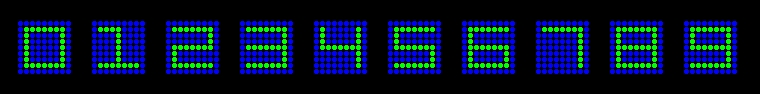
\includegraphics[width=0.99\textwidth]{pre_study_dataset}
    \caption[Straight line digits dataset]{A novel dataset created to investigate the properties of modern deep learning architectures. The dataset consists of images depicting the numbers $0-9$, each with a size of $9\times9$ pixels. The blue dots represent pixels with the value $0$; green dots represent pixels with the value $1$.}
    \figlbl{pre_study_dataset}
\end{figure}

Even in this small dataset, various features and, consequently, many net fragments exist.
It is unclear which features are learned by the network.
Regardless of what these net fragments represent, the network should have specific characteristics;
If a neuron or a group of neurons are part of a net fragment representing a feature in the input, then these neuron(s) should be strongly active if the feature is present and not or only very weakly active if the feature is not present.
Thus, different neurons should be active depending on the digit.

Digits with common characteristics should have some overlapping network activities;
For example, $7$ is contained in $3$, $3$ is contained in $9$, and $9$ is contained in $8$.
Therefore, these digits should have some common network activations.
The digit $1$, on the other hand, has nothing in common with $4$; thus, these digits should have no overlapping activations.
In the following, networks are trained, and their activations are examined for such properties.

Two types of models are trained on this dataset and examined for net fragments:
First, classification networks are used to investigate whether different architectures are more likely to contain net fragments than others.
Second, autoencoders are used to investigate whether adding constraints to the loss function can encourage net fragments.

\section{Classification}\seclbl{pre_study_classification}

\subsection{Methods}\seclbl{pre_study_classification_methods}
Different architectures are trained to investigate the emergence of net fragments in classification networks.
The models used have different feature extractors consisting of either convolutional (conv.) layers (models no. $1$-$8$, no. $11$) or fully connected (FC) layers (models no. $10$) as shown in \tabref{pre_study_models}.
Model no. $9$ has no feature extractor as the input images are so simple that they can be considered as features by themself. Model no. $10$ uses an FC layer as a feature extractor, and model no. $11$ has a Conv. layer with two hand-crafted kernels to extract horizontal and vertical lines as a feature extractor.
After the feature extractor, all models have a similar ``head'' consisting of $2$ fully connected layers.
Between each layer, a ReLU activation is employed.
The feature extractors aim to extract specific features from the images, that are combined into higher-level net fragments in the first fully connected layer of the ``head'' and composed into predictions per class (i.e. net fragments corresponding to classes) in the last fully connected layer of the ``head''.
The first FC layer of the ``head'' maps the input activations to $12$ output features.
The number of output features is determined empirically by training various architectures and examining the number of active neurons.
It was found that there are always fewer than $12$ neurons active and that, thus, this capacity is sufficient.
The last fully connected layer consists of $10$ neurons since this corresponds to the number of classes to predict.
The encoders of the models used are described in more detail in Table \tabref*{pre_study_models}.
The ``head'' is identical for all models and consists of a sequence of the following layers; FC (out size=$12$) $\rightarrow$ FC (out size=$10$) $\rightarrow$ softmax.


\begin{table}[h]
\newcolumntype{L}[1]{>{\raggedright\let\newline\\\arraybackslash\hspace{0pt}}m{#1}}
\newcolumntype{C}[1]{>{\centering\let\newline\\\arraybackslash\hspace{0pt}}m{#1}}
\newcolumntype{R}[1]{>{\raggedleft\let\newline\\\arraybackslash\hspace{0pt}}m{#1}}
    \centering
	 \begin{tabular}[t]{l L{9cm}} 
    	%\hline
    	\textbf{No.} & \textbf{Encoder Description} \\
        \hline
		1 & conv. layer (ks=$3\times3$, ch=$2$) $\rightarrow$ head \\ %\hline
		2 & conv. layer (ks=$3\times3$, ch=$4$) $\rightarrow$ head \\ %\hline
		3 & conv. layer (ks=$5\times5$, ch=$2$) $\rightarrow$ head \\ %\hline
		4 & conv. layer (ks=$5\times5$, ch=$4$) $\rightarrow$ head \\ %\hline
		5 & conv. layer (ks=$3\times3$, ch=$2$) $\rightarrow$ conv. layer (ks=$3\times3$, ch=$4$)\\
		  &  $\rightarrow$ head \\ %\hline
		6 & conv. layer (ks=$3\times3$, ch=$4$) $\rightarrow$ conv. layer (ks=$3\times3$, ch=$8$)\\
		  & $\rightarrow$ head\\ %\hline
		7 & conv. layer (ks=$3\times3$, ch=$2$) $\rightarrow$ max-pooling\\
		  & $\rightarrow$ conv. layer (ks=$3\times3$, ch=$4$) $\rightarrow$ head\\ %\hline
		8 & conv. layer (ks=$3\times3$, ch=$4$) $\rightarrow$ max-pooling\\
		  & $\rightarrow$ conv. layer (ks=$3\times3$, ch=$8$) $\rightarrow$ head\\ %\hline
		9 & head \\ %\hline
		10 & FC (in size=$9*9$, out size=$12$) $\rightarrow$ ReLU $\rightarrow$ head \\ %\hline
		11 & Hand Crafted conv. layer for vertical \& horizontal\\
		   & edge detection (ks=$3\times3$, ch=$2$) $\rightarrow$ ReLU $\rightarrow$ head \\ %\hline
    \end{tabular}
    \caption[Different classification networks investigated for net fragments]{A description of the different classification networks investigated for net fragments. A ReLU activation is employed between each layer. ``ks'' is the kernel size of a convolutional layer, and ``ch'' is the number of channels.}
    \tablbl{pre_study_models}
\end{table}

The models' parameters are optimised by minimising the cross-entropy loss with the Adam optimiser \sidecite{Kingma2015AdamAM} so that the models learn to predict the label of the images shown in \figref{pre_study_dataset}.
The learning rate is $5 \cdot 10^{-4}$, the mini-batch size is $32$ samples, and the model is trained for $10$ epochs.
After each epoch, the model's weights and activations of each layer are stored.
These vectors are visualised and investigated for net fragments.

%Furthermore, the trained models' most relevant input features are analysed.
%This analysis is done by freezing the models' parameters so that they cannot change.
%Instead, an empty image is fed into the network and updated with backpropagation of error to maximise the probability for a given class.
%This leads to the input image with the highest probability to be predicted by the model as a specific class.


\subsection{Results}\seclbl{pre_study_classification_results}
All the models learn to classify these digits perfectly within a few epochs.
Interestingly, not only the accuracy reaches $100\%$, but some models also achieve a cross-entropy loss of $0.0$, meaning that they can find a global minimum.
However, the goal is not to achieve high accuracy but to identify net fragments.
It is not feasible to visualise all activations of all layers in this thesis.
Therefore, only the activations of the second last FC layer (i.e. the first FC layer of the ``head'') after the ReLU function are shown.
This layer contains high-level net fragments that are simple to interpret\sidenote{the last layer cannot be used as it consists of $10$ neurons representing the $10$ classes}.
%Some higher-level net fragments should be visible in this layer, which are subsequently composed in the last layer to net fragments corresponding to classes.
%Interested readers who want to investigate the activations from all layers and the network weights by themselves can view an interactive visualisation at \url{http://160.85.252.38:8501}.

\figref{pre_study_activations} shows the activations of the first fully connected layer in the ``head'' of the different models.
The FC layer has $12$ neurons whose activation is indicated along the vertical axis (per model), and the horizontal axis depicts the activation of the same neuron for the classes $0$-$9$.
For example, the circle in the top left corner indicates the activation of the first neuron for class $0$, the circle in the top right corner the activation of the first neuron for class $9$, and the circle in the bottom left corner the activation of the last neuron for class $0$.
Blue circles show activations that are precisely $0$, red circles are low activations $>0$, and green circles represent strong activations\sidenote{activations $<0$ do not exist because they are set to exactly $0$ by the ReLU function}.

It can be observed that none of the models utilises all $12$ neurons, and certain neurons are always inactive regardless of the class.
Also, no obvious net fragments can be identified;
most neurons are always similarly strongly active regardless of the class.
If net fragments are formed, however, the neurons of a fragment would have to be strongly active in the presence of certain features and weakly active otherwise.
Such behaviour is not observable in these activations.

Furthermore, some images are very similar and differ in only two pixels.
Some examples are the digit pairs $5$ and $6$, $8$ and $9$, $0$ and $8$, or $3$ and $9$.
However, when the activations of the corresponding classes are compared, it is evident that almost always all activations change a little bit, and not one neuron is turned on or off, depending on the presence of these two pixels. 
This supports the assumption that typical deep learning architectures do not contain brain-like net fragments.

\begin{figure}[h]
    \centering
    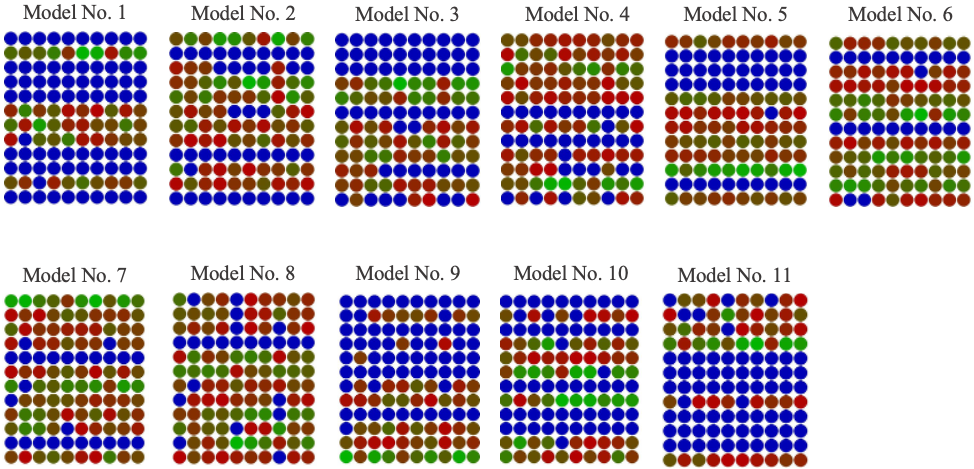
\includegraphics[width=0.99\textwidth]{pre_study_activations}
    \caption[Network activations of the classification networks]{The activations of the first fully connected layer in the ``head'' of the different networks. For each model, the activity of the $12$ neurons is shown for each class (activations along the vertical axis, classes along the horizontal axis). Red means low activation, green means high activation, and blue means activation is off (i.e. $0$).}
    \figlbl{pre_study_activations}
\end{figure}

%It can also be observed that roughly the same neurons are always active.
%For different classes, however, these neurons do not switch on or off, but the strength of the activity changes.

%\figref{pre_study_inputs_max} visualises the input that maximises the probability for each class.
%It is obvious that all models focus on the wrong features, and it can be assumed that these networks would not be robust to slight perturbations in the input.
%This also indicates that net fragments are not present in current deep learning models (or at least not to the desirable extent);
%if an object is composed of several lower-level net fragments, then some of these lower-level net fragments have to be active.
%Since these lower-level net fragments represent specific input features, corresponding pixel constellations should be visible in \figref{pre_study_inputs_max}.
%However, since the pixel combinations that maximise the probability of predicting a specific class look rather random, this suggests that pixel combinations are not composed into hierarchically more complex net fragments.

%\begin{figure}[h]
%    \centering
%    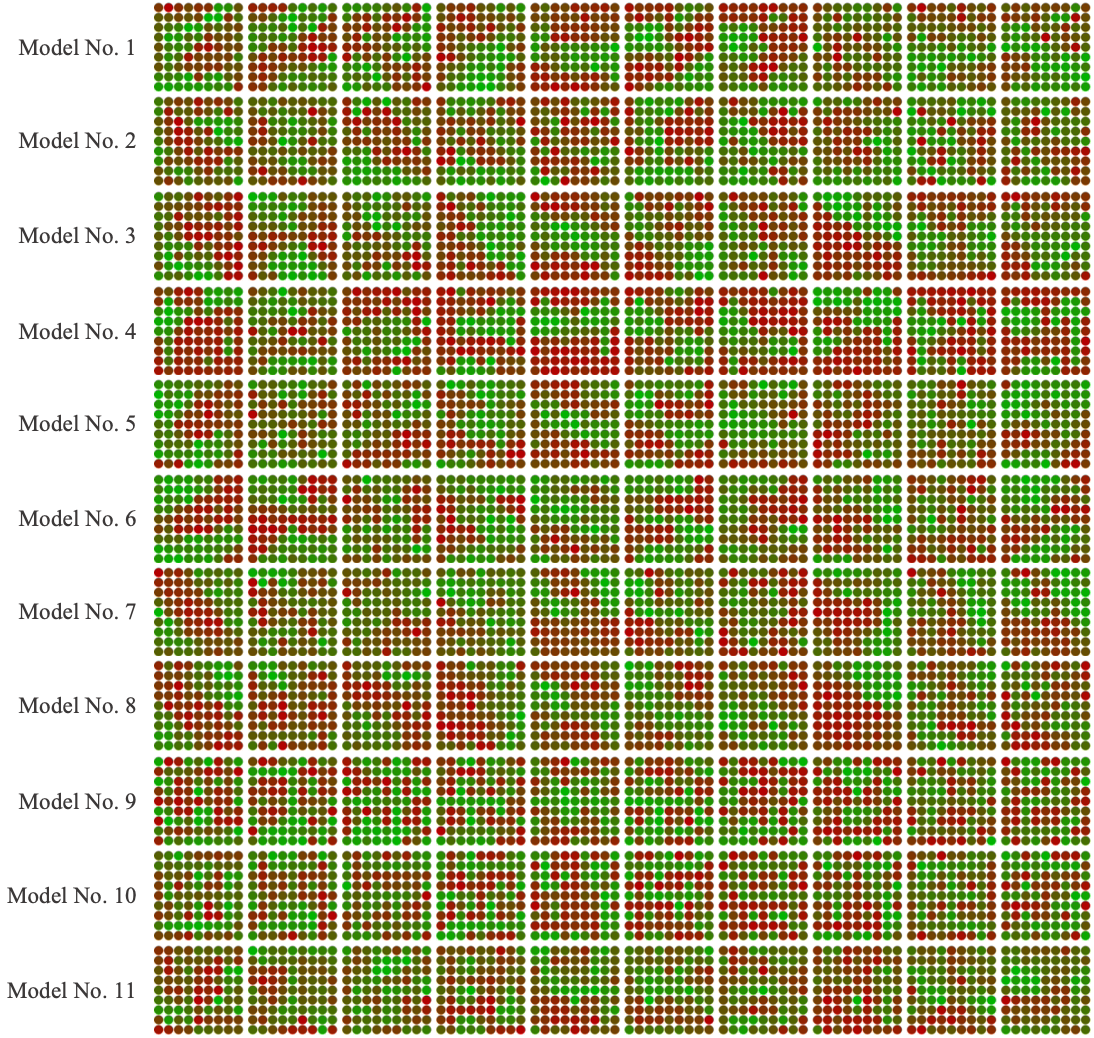
\includegraphics[width=0.99\textwidth]{pre_study_inputs_max}
%    \caption[Inputs that maximize the class output probability]{The inputs that maximize the probability that the different models predict a specific class. For example, the image in the top left corner maximizes the probability that model number $1$ predicts that this is class $0$ (digit $0$).}
%    \figlbl{pre_study_inputs_max}
%\end{figure}



\section{Autoencoders}\seclbl{pre_study_ae}

\subsection{Methods}\seclbl{pre_study_ae_methods}
Similar to the experiments with classification networks, different autoencoders are investigated.
Thereby, it is investigated if constraints in the loss function can encourage net fragments.
The analysed autoencoder architectures used are shown in \tabref{pre_study_ae_models}.


\begin{table}[h]
\newcolumntype{L}[1]{>{\raggedright\let\newline\\\arraybackslash\hspace{0pt}}m{#1}}
\newcolumntype{C}[1]{>{\centering\let\newline\\\arraybackslash\hspace{0pt}}m{#1}}
\newcolumntype{R}[1]{>{\raggedleft\let\newline\\\arraybackslash\hspace{0pt}}m{#1}}
    \centering
	 \begin{tabular}{l L{9cm}} 
    	%\hline
    	\textbf{No.} & \textbf{Encoder Description} \\
        \hline
		1 & FC (in size=$9*9$ out size=$12$) $\rightarrow$ ReLU\\
		  & $\rightarrow$ FC (in size=$12$ out size=$9*9$) \\ %\hline
		2 & FC (in size=$9*9$ out size=$40$) $\rightarrow$ ReLU\\
		  & $\rightarrow$ FC (in size=$40$ out size=$9*9$) \\ %\hline
        %\hline
    \end{tabular}
    \caption[Different autoencoders investigated for net fragments]{A description of the different autoencoder networks that are investigated for net fragments.}
    \tablbl{pre_study_ae_models}
\end{table}

The autoencoder's parameters are optimised by minimising a reconstruction loss (i.e. a distance measurement between the input and the reconstructed output) with the Adam optimiser \sidecite{Kingma2015AdamAM} so that the output looks similar to the input even though a bottleneck-layer reduces the network's capacity between encoder and decoder.
The learning rate is $5 \cdot 10^{-4}$, the mini-batch size is $32$ samples, and the model is trained for $10$ epochs.

The reconstruction loss $\mathcal{L}_{\text{rec}}$ used for the different experiments is either the L1 distance (mean absolute error) or the L2 distance (mean square error). If $\boldsymbol{x}$ is the input data with $n$ pixels and $\hat{\boldsymbol{x}}$ is the reconstructed data, then the reconstruction loss can be written as follows:


\begin{align}\eqlbl{ae_recon}
		\mathcal{L}_{\text{rec}}(\boldsymbol{x}, \hat{\boldsymbol{x}}) = \begin{cases}
      		\frac{1}{n} \sum^{n}_{i=1}|x_i - \hat{x}_i|, & \text{if L1 distance}\\
      		\frac{1}{n} \sum^{n}_{i=1} (x_i - \hat{x}_i)^2, & \text{if L2 distance}
    	\end{cases}
\end{align}

% https://debuggercafe.com/sparse-autoencoders-using-kl-divergence-with-pytorch/
As described above, activations containing net fragments should be sparse and diverse.
Therefore, a sparsity and a diversity loss are added to the reconstruction loss to encourage net fragments.
This combination of sparsity and diversity is also in line with the ideas of LeCun to obtain autonomous machine intelligence \sidecite{LeCun_AMI}.
For the sparsity loss $\mathcal{L}_{s}$, the kullback-leibler (KL) divergence is used \sidecite{10-5555-3042573-3042641}.
The hidden representations in the bottleneck are denoted as $\boldsymbol{h} = h_1, ..., h_{n_h}$.
Furthermore, the average activation probability of a neuron $h_j$ over $m$ input samples can be calculated as

\begin{align}\eqlbl{ae_kldd}
		\hat{\rho}_j = \frac{1}{m} \sum^m_{i=1} \left( \frac{1}{1+e^{-h_j}} \right)
\end{align}

where $\left( \frac{1}{1+e^{-h_j}} \right)$ is the sigmoid function that squeezes the activation in the range between $0$ and $1$. Furthermore, $\rho=0.05$ is a sparsity parameter that defines a target activation probability of each neuron. If the kullback-leibler divergence between all $\hat{\rho}_j$ and $\rho$ is minimised, an average activation probability of $\rho$ is enforced for each neuron in the hidden layer. The KL divergence is defined as:

\begin{align}\eqlbl{ae_kld}
		KL(\rho || \hat{\rho}_j) = \rho \cdot \log \frac{\rho}{\hat{\rho}_j} + (1-\rho) \cdot \log \frac{1-\rho}{1-\hat{\rho}_j}
\end{align}

The sparsity loss $\mathcal{L}_{s}$ is the sum of the KL divergence between all $\hat{\rho}_j$ and $\rho$ and thus enforces that on average only $5\%$ of the hidden representations $\boldsymbol{h}$ are active:

\begin{align}\eqlbl{ae_kldl}
		\mathcal{L}_{s}(\rho, \hat{\rho}) = \sum_{j=1}^{n_h} KL(\rho || \hat{\rho}_j)
\end{align}

Thus, this constraint ensures that the activations are sparse, consistent with the net fragments concept.
Another property of net fragments is that the activations should be diverse.
Therefore, a novel diversity loss $\mathcal{L}_{d}$ is proposed.
This loss is based on the fact that the activations $\boldsymbol{h}$ in the bottleneck layer should be as different as possible for all samples of a mini-batch $(\boldsymbol{x}^{(1)}, ..., \boldsymbol{x}^{(m)})$.
The sum of the dot product between the activation of a sample $\boldsymbol{h}^{(i)}$ and all other samples $\boldsymbol{h}^{(j)}$, for $i \neq j$ is small if the samples within a batch have a high diversity. Therefore, the diversity loss can be defined as:

\begin{align}\eqlbl{ae_kldl2}
		L\mathcal{L}_{d}(\boldsymbol{z}) = \frac{1}{n} \sum_{i=1}^n\sum_{j=1}^{n_h} \boldsymbol{h}^{(i)} \cdot \boldsymbol{h}^{(j)}, \text{ if } i\neq j
\end{align}

Minimising $\mathcal{L}_{d}$ leads to diverse activations in the bottleneck layer. 
The overall loss can be defined as the sum of these three loss components, with $\lambda_s$ and $\lambda_d$ being hyperparameters that control the influence of the diversity and sparsity loss.

\begin{align}\eqlbl{ae_kldl3}
		L = L_{\text{rec}} + \lambda_s \cdot L_{s} + \lambda_d \cdot L_{d}
\end{align}

In the experiments, these hyperparameters were set to $\lambda_s = 0.02$ and $\lambda_d = 0.02$, respectively $\lambda_s = 0$ and $\lambda_d = 0$ if the sparsity and diversity loss should not be used.
Similar to the analysis of classification architectures, the model's activations of each layer are stored after every epoch.
These vectors are visualised and investigated for net fragments.

\subsection{Results}\seclbl{pre_study_ae_results}
The activations of the autoencoders trained with reconstruction loss only and without diversity or sparsity constraint (i.e. $\lambda_s = 0$ and $\lambda_d = 0$) look very similar to those of the classification network; about half of the neurons are always active regardless of the object depicted in the image, and the other half of neurons are always inactive. Thus, this version of the autoencoder has the same problem as the classification networks. Adding a sparsity constraint (i.e. $\lambda_s = 0.02$ and $\lambda_d = 0$) improves this issue slightly. The activations become sparse, but the same neurons are always active independent of the objects in the image. Only in a few cases can a set of neurons be identified that represents specific objects or features.

However, if all three loss components are used, the activations look much better. In this case, specific neuron combinations represent object-dependent features and are only active for specific objects. There are no more neurons that are constantly active. It is even possible to infer image labels based on a binary activity state (i.e. which neuron is active or inactive) without knowing the strength of the activation, even though labels are not used during training. Thus, an autoencoder with additional sparsity and diversity constraint can represent net fragments to some extent\sidenote{except that constraint 1, which says that net fragments span several layers by design, is violated (c.f. \secref{neuro_concepts_net_fragments})}.


\begin{figure}[h]
    \centering
    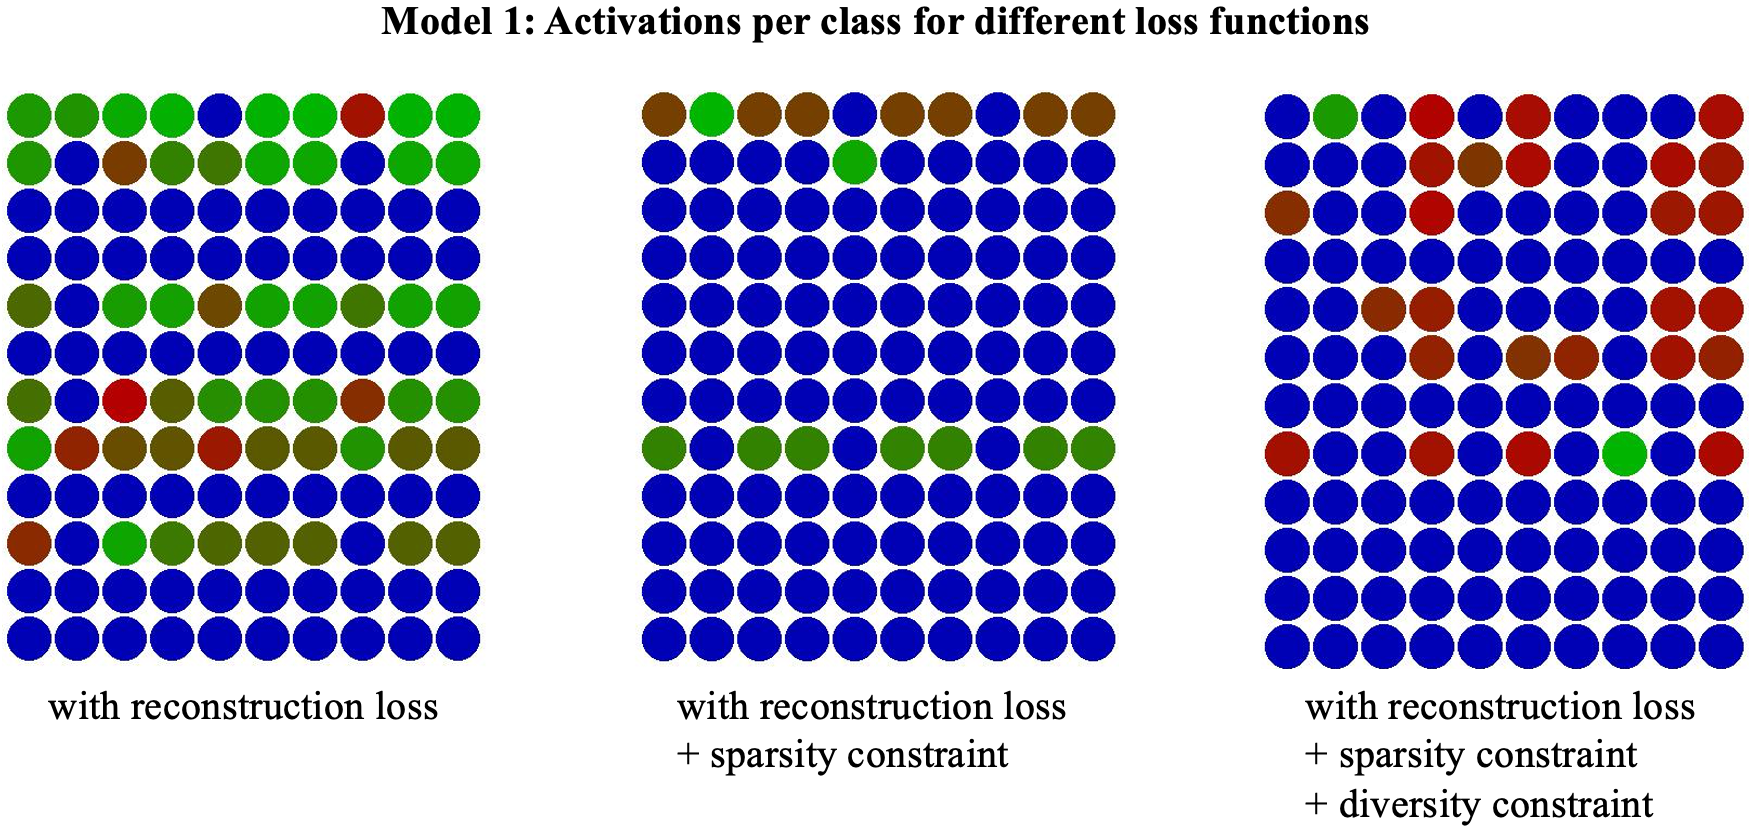
\includegraphics[width=0.99\textwidth]{pre_study_ae1}
    \caption[Network activations of the smaller autoencoder model]{The activations in the bottleneck layer of the smaller autoencoder ``model 1'' for different loss functions. For each loss function, the activity of the $12$ neurons in the bottleneck layer is shown for each class (activations along the vertical axis, classes along the horizontal axis). Red means low activation, green means high activation, and blue means activation is off (i.e. $0$).}
    \figlbl{pre_study_ae1}
\end{figure}

\figref{pre_study_ae1} shows the activations of the ``model 1''.
On the left are the activations without constraint, in the middle are the activations with sparsity constraint and on the right are the activations with sparsity and diversity constraints.
For each of these three loss functions, the activations in the bottleneck layer are shown per class (activations along the vertical axis and classes along the horizontal axis).
It is observable that adding sparsity and diversity constraints gives more meaning to the individual neurons: While the same neurons are always active  without both constraints, the activations are significantly more varied between the classes when both constraints are used.
This becomes even more obvious when the activations of the bigger autoencoder ``model 2'' are investigated (c.f. \figref{pre_study_ae2} (a)).

\begin{figure}[h]
    \centering
    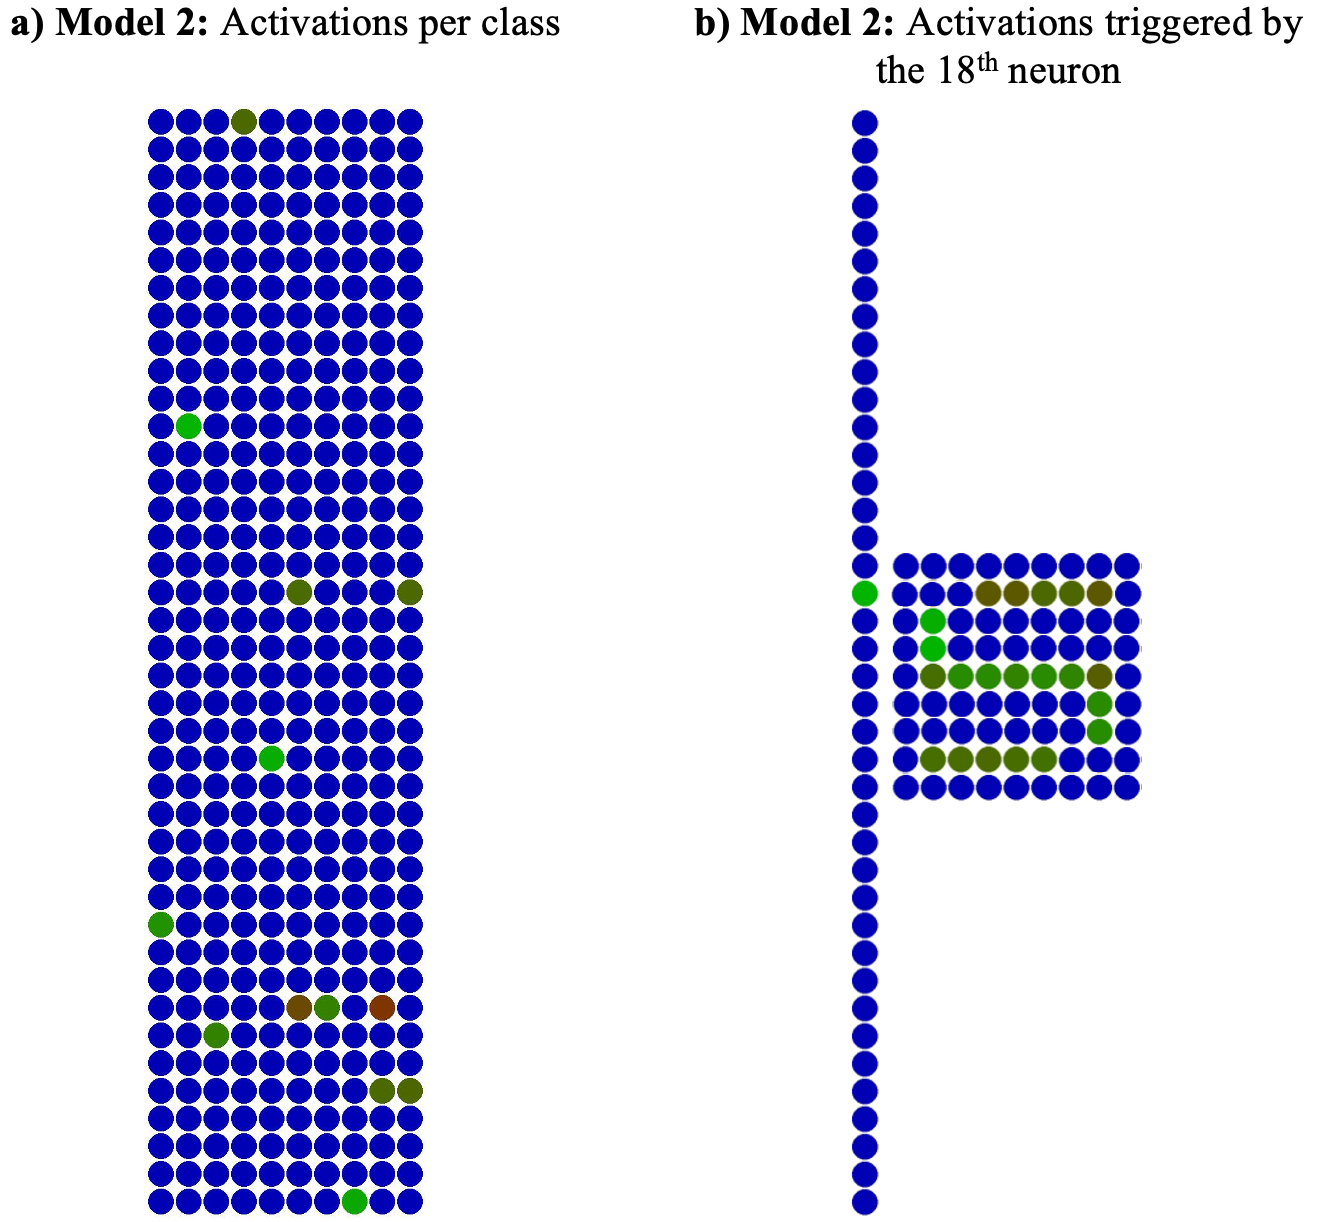
\includegraphics[width=0.99\textwidth]{pre_study_ae2}
    \caption[Network activations of the bigger autoencoder model]{On the left side (a), the activations in the bottleneck layer of the bigger autoencoder ``model 2'' are shown. The activity of the $40$ neurons in the bottleneck layer is shown for each class (activations along the vertical axis, classes along the horizontal axis). On the right side (b), the output of the decoder is shown when the 18th neuron is set to $1$, and all other neurons are set to $0$. The $18$-th neurons is a feature that is needed to generate the numbers $5$ and $9$.}
    \figlbl{pre_study_ae2}
\end{figure}

It is also examined what features the various neurons in the bottleneck layer represent.
This is done by manually creating a bottleneck activation $\boldsymbol{h} = h_1, ..., h_{n_h}$ and feeding it through the decoder.
To examine which feature the $i$-th neuron represents, $h_i$ is set equal $1$ and all other neurons are set equal $0$.
\figref{pre_study_ae2} (b) shows which feature the $18$-th neuron represents. Together with the $33$-th neuron, this neuron represents the number 5 and the $36$-th neuron, the number 9.
Thus, it is a feature (i.e. a net fragment) that assembles with other features to represent an object.

\section{Conclusion}\seclbl{pre_study_conclusion}
Different architectures have been trained with different targets on a very simple and easily interpretable dataset.
The network activations are tracked during training and analysed for net fragments.
Typical vision architectures are sequential and build up a composition of features (i.e. net fragments) over several layers.
Usually, the embeddings of a pre-defined layer are used for downstream tasks such as classification.
Autoencoders typically use the bottleneck layer, a classification networks typically have a classification head (i.e. a FC layer with a Softmax activation) after the last encoder layer and thus extract these embeddings from the last model layer.
Therefore, embeddings are extracted from one layer.
Net fragments, on the other hand, span over multiple layers\sidenote{net fragments can be thought of as the ``path'' of features through a network} and hence this principle is violated.

Furthermore, net fragments are strongly activated when the corresponding feature they represent is present in the input and are weakly active or not active at all when it is not present.
Typical deep learning networks have neurons that are never active, while the active neurons usually remain active regardless of the input data and only change their activity strength.
Thus, the information about different features is not distributed on different neurons but transported as activation strength of neurons through the network.
Therefore, deep learning architectures do not comprise brain-like net fragments by default.

However, adding a sparsity and diversity constraint alleviate this issue:
Adding such constraints to the loss function encourages neurons to represent specific features typical for a subset of the objects.
